% tools voor document
\documentclass{article} % definieer type document (article, resume, etc...)
\usepackage[english]{babel} % definieer taal van document

\usepackage[a4paper,top=2cm,bottom=2cm,left=5cm,right=5cm,marginparwidth=1.75cm]{geometry} % definieer formaat van document

% Handige packages
\usepackage{imakeidx} % package om indices te maken
\usepackage{amsmath} % package voor formules
\usepackage{graphicx} % package voor het invoegen van images
\usepackage{listings} % package voor het invoegen van listings (bron code)
\usepackage[colorlinks=true, allcolors=blue]{hyperref} % package voor hyperlinks (intern als extern)
\usepackage{xcolor} % package voor standaard kleuren
\usepackage{parskip} % package voor het formateren van paragraven
\usepackage{multirow} % package voor formateren tabellen --- \multicolumn{x}{|c|}{tekst}
\usepackage{ulem} % package om zinnen door te strepen met \sout{}
\usepackage[many]{tcolorbox} % for COLORED BOXES (tikz and xcolor included)

\usepackage[sorting=none, style=nature]{biblatex} %Imports biblatex package
\usepackage{csquotes}
\addbibresource{references.bib} %Import the bibliography file

% definieer kleuren: {naam}{kleurstijl}{waardes}
\definecolor{codegreen}{rgb}{0,0.6,0}
\definecolor{codegray}{rgb}{0.5,0.5,0.5}
\definecolor{codepurple}{rgb}{0.58,0,0.82}
\definecolor{backcolour}{rgb}{0.95,0.95,0.92}

% definieer stijl van lijsten
\lstdefinestyle{mystyle}{
    backgroundcolor=\color{backcolour},   
    commentstyle=\color{codegreen},
    keywordstyle=\color{magenta},
    numberstyle=\tiny\color{codegray},
    stringstyle=\color{codepurple},
    basicstyle=\ttfamily\footnotesize,
    breakatwhitespace=false,         
    breaklines=true,                 
    captionpos=b,                    
    keepspaces=true,                 
    numbers=left,                    
    numbersep=5pt,                  
    showspaces=false,                
    showstringspaces=false,
    showtabs=false,                  
    tabsize=2
}
\lstset{style=mystyle} % verander standaard stijl naar eigen stijl

\newtcolorbox{boxA}{
    fontupper = \bf,
    boxrule = 1.5pt,
    colframe = black % frame color
}

\hypersetup{
    colorlinks=true,
    linkcolor=blue,
    filecolor=magenta,      
    urlcolor=cyan,
    }
\urlstyle{same}

\begin{document}
%%%%%% TITLE PAGE %%%%%
\sffamily
\begin{titlepage}
    \centering
    \vfill
    {\bfseries\Huge
    Groepsverslag Tinlab Advanced Algorithms \\
    \vskip2cm
    }
    {\bfseries\Large
    Thijs Dregmans, Tobias de Bildt, Eliam Traas, Hidde-Jan Daniëls\\
    }
    {
    \bfseries\normalsize
    1024272, 1023603, 1003233, 0943798\\
    \vskip1cm
    \today\\
    }    
    \vfill
    
\includegraphics[width=4cm]{logohr.png} % also works with logo.pdf
    \vfill
    \vfill
\end{titlepage}
\newpage

%%%%% TABLE OF CONTENTS %%%%%
\tableofcontents
\newpage

%%%%% ANALYSE %%%%%
\section{Analyse}
Uit een analyse van het ministerie van Infrastructuur en Waterstaat (IenW) blijkt dat een groot aantal sluizen in Nederland de komende jaren aan renovatie toe zijn. De minister van Infrastructuur heeft opdracht gegeven voor het modelleren van sluizen om een beter beeld te krijgen van benodigde ont- werpkeuzes met betrekking tot - onder andere - veiligheid, efficiëntie, capaciteit, onderhoudskosten en duurzaamheid. Voordat requirements worden opgesteld, volgt een algemene analyse van het Nederlandse sluizenpark. \par

\subsection{Sluizen in Nederland}
Het Nederlandse sluizenpark bestaat uit een breed scala aan verschillende soorten sluizen. Het gaat niet alleen over sluizen voor de profesionele scheepvaart, maar bijvoorbeeld ook sluizen voor militaire doeleinden. Een voorbeeld hiervan is de \textit{'Plofsluis'} bij Nieuwegein. \cite{rijkswaterstaatPlofsluis} Sluizen met een militaire functie, zoals de Plofsluis, zijn vooral iets van het verleden. \par

Sluizen zijn in te delen in drie categorieën:
\begin{enumerate}
    \item Sluizen voor waterhuishouding
    \item Sluizen voor de scheepvaart
    \item Sluizen met een militaire functie
\end{enumerate}

\subsection{Soorten sluizen}
Vaak hebben sluizen meerdere functies. Het is dan bijvoorbeeld een grote sluis voor de scheepvaart, maar wordt ook gebruikt voor het watermanagement.\par

Onder de verschillende categorieën - die in feite functies van sluizen zijn - vallen een aantal typen. Voor de waterhuishouding bestaan er bijvoorbeeld zogenaamde ‘uitwateringssluizen’, ‘Ontlastsluizen’, ‘irrigatiesluizen’ en ‘keersluizen’. \par

De keersluis is een voorbeeld, waarbij de verschillende functies overlappen. Keersluizen worden vaak bij zeehavens aangelegd. Als het water te laag komt te staan, dan kan de keersluis worden gesloten om schade aan de haven en schepen door laag water worden voorkomen. De keersluis kan ook voor het omgekeerde gebruikt worden. Het heet dan een ‘doksluis’. In een dok worden schepen droog gebouwd. Met eb - als de dok droogstaat - wordt de sluis(deur) gesloten, zodat het water met hoogwater niet binnenkomt. Een keersluis heeft dus zowel een functie voor de waterhuishouding als voor de scheepvaart. \par

\subsection{Schutsluizen}
Het meest van de eerder genoemde sluizen kenmerkt zich door de enkele deuren. Hoewel het dus voorkomt dat een sluis voor de scheepvaart een enkele deur heeft - zoals de keersluis - zijn de meeste sluizen voor de scheepvaart schutsluizen. Schutsluizen kenmerken zich door de dubbele deuren. Ze verbinden twee waterwegen die een ongelijk waterpeil hebben. Door de deuren beurtelings te sluiten, water van de hoger gelegen waterweg naar binnen te pompen en de hoger gelegen deuren te openen, kunnen schepen eenvoudig over waterwegen getransporteerd worden, terwijl die waterwegen een ongelijk waterpeil hebben \cite{Arends1994}. \\
In de scheepvaart zijn de vrijwel alle sluizen, schutsluizen. Daarom ligt de focus in dit onderzoek op schutsluizen.
\newpage

\subsection{Werking van een schutsluis}
Een schutsluis heeft een aantal fases:
\begin{enumerate}
    \item Het schip vaart/de schepen varen de sluis binnen.
    \item De sluiskolk wordt gevuld of leeggepompt.
    \item Het schip vaart/de schepen varen de sluis uit.
\end{enumerate}
Bij een schutsluis zijn er minimaal 2 sluisdeuren. Ten alle tijde is er tenminste één deur gesloten. Anders zou het hebben van meerdere deuren zinloos zijn.

\subsubsection{Proces}
Er is sprake van een lager gelegen waterweg en een hoger gelegen waterweg. De lager gelegen waterweg noemen we \textbf{‘beneden’} en de hoger gelegen waterweg \textbf{‘boven’}.

\begin{boxA}
    \begin{itemize}
        \item In fase 1 is de bovenkant van de sluis gesloten. Beneden is geopend. Omdat de lagere deur geopend is, is het waterpeil in de sluis gelijk aan dat van het water stroomafwaarts.
        \item In fase 2 worden beide deuren gesloten. Het water in de sluis wordt op gelijke hoogte gebracht met dat stroomopwaarts.
        \item Als het water in de sluis op gelijke hoogte is als dat met het water stroomopwaarts, dan start fase 3. In fase 3 worden de sluisdeuren boven geopend en kan het schip de sluis uitvaren.
    \end{itemize}
\end{boxA}

Dit proces kan ook omgedraaid worden. In dat geval komt het schip de sluis van boven aanvaren. De sluisdeur boven gaat open wanneer het waterpeil gelijk is met dat van boven. Het schip vaart naar binnen. Het waterpeil in de sluis wordt gelijk gemaakt met dat van het water beneden. Vervolgens kunnen dan de sluisdeuren beneden open om het schip toegang tot de lager gelegen vaarweg te verlenen. \par

\subsubsection{Waterpeil bijstellen}
Water verplaatsen van boven naar beneden is niet moeilijk. Water stroomt van nature naar het laagste punt. Dit principe wordt in de sluizen gebruikt. Bij veel sluizen zijn er in de sluisdeuren luiken gemaakt, die tijdens fase 2 geopend kunnen worden. Door deze luiken te openen, kan er water vanuit de hoger of lager gelegen waterweg water naar of van de sluis worden gepompt. \par

\newpage
\subsubsection{Flowchart werking sluis}
Voor het ontwerpen van de sluis zal er gekeken moeten worden naar de vorige hoofdstukken. Voor een wat duidelijkeroverzicht is de volgende flowchart gevonden om als referentie te gebruiken voor het model. \par
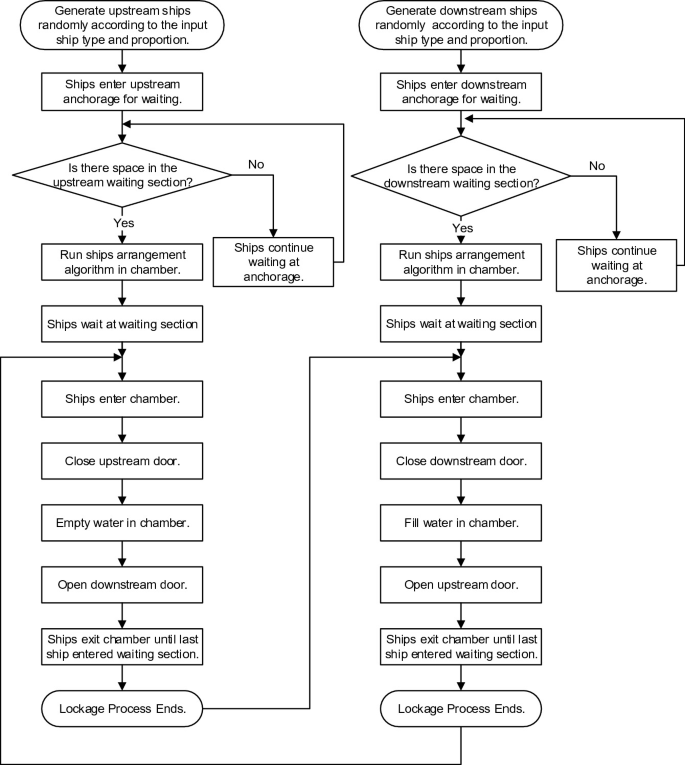
\includegraphics[width=0.9\textwidth]{lockageprocess.png} \\ \cite{flowchart1}
\newpage

\subsection{Onderdelen van een schutsluis}
Een eenvoudige schutsluis bestaat uit enkele onderdelen:
\begin{enumerate}
    \item Sluisdeuren voor de afsluiting tussen sluis en waterweg stroomopwaarts.
    \item Sluisdeuren voor de afsluiting tussen sluis en waterweg stroomafwaarts.
    \item Luiken in de sluisdeuren stroomt opwaarts.
    \item Luiken in de sluisdeuren stroomafwaarts.
\end{enumerate}
De Grevelingensluis heeft een breedte van 16 meter en een lengte van 139 meter. Er mogen schepen in die minder dan 110 meter lang zijn. Dit wordt ook wel de \textbf{‘schutlengte’} genoemd. \cite{WaterkaartGrevelingensluis}

\subsection{Bediening van schutsluizen}
Bedieningstijden zijn veelal online te vinden. Rijkswaterstaat heeft een speciale website met reguliere openingstijden. Daarnaast is het vaak mogelijk om buiten deze tijden een afspraak te maken voor gebruik maken van een sluis. Als voorbeeld, in de sluisplanning van de volkeraksluizen valt af te lezen dat het ongeveer 20 á 30 minuten duurt. \cite{vaarweginformatie, volkeraksluizen, SluisplanningVolkeraksluizen} \par 

Wat betreft tijden, neemt fase 2 het grootste deel van de tijd in beslag. In een grote sluis zoals de Volkaraksluizen - waar jaarlijks zo’n 150.000 vrachtschepen passeren - worden in een paar minuten bijna 900.000\footnote{De sluis is 16 meter breedte en 139 meter lang. Er is een hoogte verschil van 0.40 meter. 0.4 * 16 * 139 = 889 kubieke meter.} liters water verplaatst. \cite{WaterkaartVolkeraksluizen} Geschat wordt dat fase 2 zo’n 20 tot 25 minuten duurt, terwijl fase '1 en 3' 1 tot 3 minuten duren. \par

Na aanleiding van deze analyse definiëren wij de requirements, in lijn met de eisen gesteld door de opdrachtgever. \par

\newpage

%%%%% REQUIREMENTS
\section{Requirements}
De opdrachtgever heeft gesteld dat het doel is om tot een model van een volledig automatische sluis te komen. Hierbij wordt gehoopt op een verbetering in:
\begin{enumerate}
    \item Veiligheid
    \item Efficientie
    \item Duurzaamheid
\end{enumerate}

\subsection{Veiligheid}
We definiëren veiligheid als de afwezigheid van gevaar voor mens en bezit. De volgende situaties zijn gevaarlijk voor mens en/of bezit:
\begin{itemize}
    \item Beide deuren (boven en onder) zijn op hetzelfde moment geopend of zijn op hetzelfde moment in beweging. Dit zorgt - door het waterpeil verschil tussen boven en onder - voor een niet te stoppen stroom aan water. Dit kan voor gevaar zorgen.
    \item Een deur sluiten terwijl er een schip - of iets dergelijks - in de deuropening ligt.
    \item Een deur openen terwijl het waterpeil aan beide kanten van de deur ongelijk is. Dit zorgt voor een gevaarlijke stroom aan water - die vergelijkbaar is met punt 1.
    \item We willen voorkomen dat schepen tegen elkaar varen bij het in- en uitvaren van de sluis. Ook mag een schip niet tegen een sluisdeur varen. Er moeten seinen (stoplichten) aanwezig zijn voor de schepen die aangeven wanneer de schepen de sluis in of uit mogen varen.
\end{itemize}

\subsection{Efficientie}
Efficiëntie is de manier waarop de sluis werkt tenopzichte van de locatie van schepen buiten de sluis. Dit uit zich in:
\begin{itemize}
    \item Als een schip buiten de sluis gedetecteerd wordt waar de sluisdeur open gaat, zal de deur niet dicht moeten gaan om weer open te gaan voor dat schip.
    \item In een situatie waar schepen aan beide kanten tegelijkertijd aankomen, zal het schip aan de kant van waterniveau voorrang krijgen op het schip aan de andere kant.
\end{itemize}

Om de efficiëntie te maximaliseren wordt door de sluis gekeken naar wachtende schepen. De sluis geeft voorrang aan het schip aan de kant van de sluis waar de deur geopend is. Als een schip aan de kant waar het waterniveau ander is komt, zal de sluis dit schip voorrang geven. \\
Om de efficiëntie verder te verhogen, neemt de sluis de kleinst mogelijke hoeveelheid tijd om zowel de deuren te openen, te sluiten en de schepen naar binnen en naar buiten te laten varen.

\subsection{Duurzaamheid}
Duurzaamheid is ‘een ontwikkeling die voorziet in de behoeften van de huidige generatie, zonder de behoeften van toekomstige generaties, zowel hier als in andere delen van de wereld, in gevaar te brengen’. \cite{CBSduurzaamheid} \par

Dit heeft betrekking op de materiaalkeuze tijdens de bouw van de sluis. Omdat het model slechts een symbolische representatie van de sluis is, kan geen invloed worden uitgeoefend op de materialen. Daarom laten we de materiaalkeuze buiten beschouwing. \\
Een verbeterde duurzaamheid kan ook opgevat worden als het gebruik van een minimale hoeveelheid energie. Een sluis gebruikt energie voor verschillende zaken waarvan de belangrijkste de aansturing van de deuren en de pompen zijn. \\
Hoewel dit geen invloed heeft op het model, kunnen we energie besparen door pompen te vervangen door sluisluiken.
\newpage


\subsection{Functionele requirements}
Bovengenoemde eisen zijn omgezet in de volgende functionele requirements:
\begin{enumerate}
    \item Er kan nooit een situatie ontstaan waarin niet ten minste één deur is gesloten.
    \item Een deur kan nooit gesloten worden, als er een schip in de deuropening ligt.
    \item Een deur kan nooit geopend worden, als het waterpeil aan beide kanten van de deur ongelijk is.
    \item Het invaarsein mag enkel en alleen op groen staan, als de bijbehorende deur geopend is en het uitvaarsein op rood staat.
    \item Het uitvaarsein mag enkel en alleen op groen staan, als de bijbehorende deur geopend is en het invaarsein op rood staat.
    \item Er kan op elk gegeven moment slechts één sein op groen staan.
    \item Als er een schip in de sluis zit, zal er ergens een deur openen, zodat een schip nooit oneindig vast kan komen te zitten.
\end{enumerate}
\newpage

%%%%% MODELEREN %%%%%
\section{Modeleren}

\subsection{Modelcriteria van Vaandrager}

Uit het verslag van Frits Vaandrager is af te leiden dat goede modellen bouwen erg belangrijk is. Frits durft het zelfs kunst te noemen. Voor het maken van goede modellen zijn er 7 criteria. Deze criteria zijn vaak lastig aan te houden, maar een goed model houdt meestal alle criteria aan. De 7 criteria die Frits noemt, kunnen als volgt worden uitgelegd:
\begin{itemize}
    \item Een goed model moet duidelijk een object modelleren. 
    \item Een goed model moet een duidelijk en specifiek doel hebben en moet bijdragen aan de realisatie van dat doel. 
    \item Een goed model is traceerbaar, wat inhoudt dat elk element van het model correspondeert met het object dat je modelleert. 
    \item Een goed model is een model waar de eigenschappen van het gemodelleerde object overeenkomen met de werkelijkheid. 
    \item Een goed model moet eenvoudig zijn, maar niet te eenvoudig. Mensen houden over het algemeen wel van eenvoud.Dit moet niet ten koste gaan van de functionaliteit van het model. 
    \item Een goed model moet de mogelijkheid bieden voor uitbreiding en hergebruik. Het moet ontworpen zijn met het oog op evolutie, omdat technologie voortdurend vooruitgang boekt.
    \item Een goed model moet goed kunnen integreren met andere modellen, omdat projecten vaak uit verschillende onderdelen bestaan die meerdere modellen vereisen.

\end{itemize}
De modelcriteria van Vaandrager zijn vaak tegenstrijdig, omdat het ene criterium van een model vaak ten koste gaat van het andere criterium. Een voorbeeld hiervan is dat het streven naar eenvoud in een model de traceerbaarheid ervan kan verminderen. Het eenvoudig repliceren van het object kan de complexiteit van het model vergroten en de eenvoudigheid dus verminderen.

\subsection{Onderdelen model van sluis}

Om de criteria van Vaandrager zo veel als mogelijk te handhaven, is gekozen voor een model dat de volgende onderdelen heeft.
\begin{itemize}
    \item sluisdeur
    \item sluisluik
    \item schipsensor
    \item vaarsein
    \item sluis (controller)
\end{itemize}

Met deze onderdelen in het Uppaal model, is getracht het derde criterium te handhaven: Een goed model moet traceerbaar zijn.
\newpage

\subsection{Werking model van sluis}

\subsubsection{Sluisdeur}

Een sluisdeur heeft 4 states:

\begin{itemize}
    \item 'gesloten' \\
        Dit is de intial state. In deze state is de deur gesloten. Er is een transitie mogelijk naar 'aanHetOpenen'.
    \item 'aanHetOpenen' \\
        De transitie naar deze state wordt gesynchroniseerd met de Sluis controller. De clock wordt gereset, in de transitie. In deze state zijn de deuren aan het openen. Het openen van de deur kost 2 minuten. (Zie paragraaf 1.6) Met Guards en een Invariant, wordt dit bereikt.
    \item 'open' \\
        De transitie naar deze state wordt weer gesynchroniseerd met de Sluis controller. In deze state kan een schip naar binnen of naar buiten varen. Wanneer de Sluis controller dat besluit, wordt een transitie genomen naar 'aanHetSluiten'.
    \item 'aanHetSluiten' \\
        In deze state is de sluisdeur aan het sluiten. Dit kost opnieuw weer 2 minuten. Na 2 minuten (in het model) wordt een transitie genomen naar 'gesloten' -- de initial state. Ook deze transitie is gesynchroniseerd met de Sluis controller, zodat de controller zeker weet dat de deur daadwerkelijk gesloten is, voordat het bijvoorbeeld de luiken opent. 
    
\end{itemize}

\begin{figure}[h]
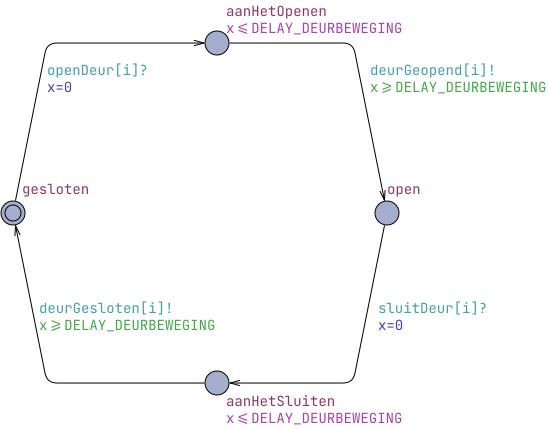
\includegraphics[width=5cm]{sluisdeur.png}
\centering    
\caption{sluisdeur}
\end{figure}
% Import image, give figure no. and center image

Er is gekozen voor een sluisdeur met 4 states om de overeenkomsten met de werkelijkheid zoveel mogelijk te behouden. Dit zorgt ervoor dat ingeleverd wordt op de eenvoud van het model, maar na afweging is besloten tot 4 states om het model realistisch te houden. Het kost immers twee minuten om de deuren te openen. Dit is een fundamenteel feit van een sluis en hoort dus in het model te zitten. \\
De gemodeleerde sluis bevat twee sluisdeuren -- één aan de 'hoge' kant en één aan de 'lage' kant. Dit wordt in Uppaal geïmplementeerd door een geparameteriseerde deur.

\newpage

\subsubsection{Sluisluik}

In het kader van duurzaamheid is gekozen voor een set van luiken in plaats van pompen. (Zie paragraaf 2.3) Ook deze zijn -- net al de deuren -- geparameteriseerd. \\
Een sluisluik heeft twee states:

\begin{itemize}
    \item 'gesloten' \\
        Dit is de intial state. In deze state is het luik gesloten. Er is een transitie mogelijk naar 'geopend'. Deze transitie wordt gesynchroniseerd met de Sluis controller.
    \item 'geopend' \\
        In deze state is het luik geopend. Er is een transitie mogelijk naar 'gesloten'. Deze transitie wordt gesynchroniseerd met de Sluis controller.
\end{itemize}

\begin{figure}[h]
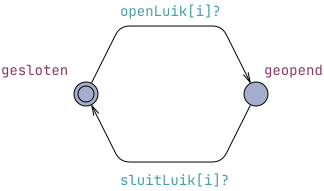
\includegraphics[width=5cm]{sluisluik.png}
\centering    
\caption{sluisluik}
\end{figure}
% Import image, give figure no. and center image

In de sluisdeuren is gekozen voor een extra twee states voor het 'aanHetOpenen' en 'aanHetSluiten' van de deuren. Hoewel dit is ook mogelijk is voor de luiken, is de conclusie getrokken dat dit minder waarde heeft. Ten eerste, omdat als gekozen zou worden voor twee extra states, de duur van het openen en sluiten betrekkelijk laag is. Denk aan bijvoorbeeld 0,5 minuten. Daarnaast is het voor het model minder relevant, om de tijdsduur van het openen en sluiten van de luiken mee te nemen. Om het overzichtelijk te houden, blijft het bij twee states. \\
In ons model hoort bij elke deur, een luik. Omdat de deuren geparameteriseerd zijn, zijn de luiken op zo'n zelfde manier geparameteriseerd.

\subsubsection{Scheepssensor}

\begin{figure}[h]
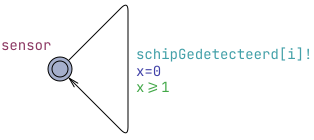
\includegraphics[width=5cm]{schipsensor.png}
\centering    
\caption{schipsensor}
\end{figure}
% Import image, give figure no. and center image

Het doel van een scheepssensor is het detecteren van schepen. Deze template heeft slechts één state en één transitie naar zichzelf. Deze transitie is gesynchroniseerd op het kanaal 'schipGedetecteerd' met de Sluis controller. \\
De template bevat een clock, update en Guard om Zeno gedrag te voorkomen. \par

Er zijn in het model dus twee deuren en twee luiken. Om de sluis te automatiseren, wordt gebruik gemaakt van scheepssensoren. In het model zijn er drie sensoren: Één buiten de sluis aan de 'hoge' kant, één buiten de sluis aan de 'lage' kant en één binnen in de sluis. Door deze combinatie van sensoren kan de sluis detecteren waar er een schip is. 

\newpage

\subsubsection{Vaarsein}

Een vaarsein kan op 'rood' of op 'groen' staan. Met de kanalen 'zetSeinOpGroen' en 'zetSeinOpRood' zijn de twee transities gesynchroniseerd met de Sluis controller.

\begin{figure}[h]
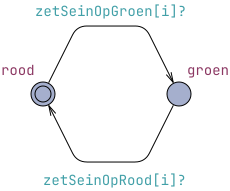
\includegraphics[width=4cm]{vaarsein.png}
\centering    
\caption{vaarsein}
\end{figure}
% Import image, give figure no. and center image

\newpage

\subsubsection{Sluis controller}

De Sluis controller heeft de leiding en neemt op basis van de sensoren actie.

De states zijn in clusters in te delen:

\begin{itemize}
    \item Schip vaart naar laag binnen.
    \item Water wordt naar hoog niveau gebracht.
    \item Schip vaart naar buiten hoog.
    \item Water wordt naar laag niveau gebracht.
    \item Schip vaart naar hoog binnen.
    \item Schip vaart naar buiten laag.
\end{itemize}

\begin{figure}[h]
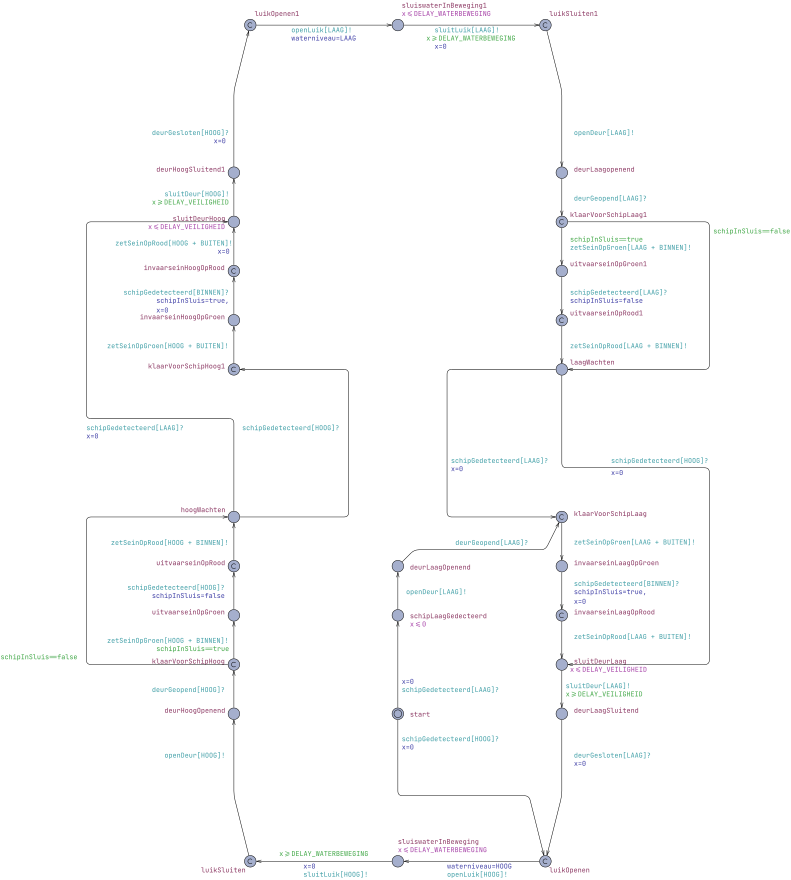
\includegraphics[width=\linewidth]{sluis.png}
\centering    
\caption{Sluis (controller)}
\end{figure}
% Import image, give figure no. and center image

In het begin -- in de initial state -- is het waterniveau laag en alle deuren gesloten. Ofwel er wordt een schip hoog gedetecteerd, of er wordt een schip laag gedetecteerd. \par

In de onderste en bovenste drie wordt het sluiswater bewogen. Een luik wordt geopend. Wacht het systeem tot 15 minuten verstreken zijn. Daarna wordt het luik gesloten en kan het systeem het schip weer in of uit de sluis laten varen. \\
Op basis van de behoefte -- welke sensor getriggerd wordt -- bepaalt de controller of de vaarseinen op groen gaan of dat de deuren sluiten en de luiken open gaan. \\
Als er geen schip in de sluis zit zal er bijvoorbeeld geen vaarsein binnen op groen gaan.

\newpage

\subsection{Beperkingen}

Door bepaalde ontwerpkeuzes zijn er in het model verschillende beperkingen gekomen. \par

Er zijn een aantal states waarin het model wacht op input van sensoren:

\begin{itemize}
    \item 'start'
    \item 'hoogWachten'
    \item 'laagWachten'
\end{itemize}

In deze states is het model in een 'idle' state waarin het model schepen zowel hoog als laag kan detecteren. Enkel het schip wat als eerst wordt gedetecteerd, wordt gezien. Als de sluis eenmaal in bedrijf is, en het water is aan het stijgen, dan is de sluis 'blind'. Het luistert niet naar de sensoren. Door de manier waarop de sensoren zijn gebouwd -- met één state -- is er ook geen geheugen mogelijk. Een detectie is een edge die \(dx=0\) duurt. \\
Door deze beperking is het niet mogelijk om meerdere schepen in overweging mee te nemen. We versimpelen ons model tot één enkel schip per cyclus.

\newpage

%%%%% VERIFICATIE %%%%%
\section{Verificatie}

Met behulp van de Uppaal tool, konden de meeste requirements geverifeerd worden. (Zie paragraaf 2.4)

\subsection{Er kan nooit een situatie ontstaan waarin niet ten minste één deur is gesloten.}

Deze requirement is in Uppaal geverifeerd met de volgende CTL query:

\begin{boxA}
    $A[]$ $exists(i:sluisdeur\_id)$ $sluisdeur(i).gesloten$
\end{boxA}

Uppaal heeft geverifeerd dat het systeem voldoet aan deze requirement.

\subsection{Een deur kan nooit gesloten worden, als er een schip in de deuropening ligt.}

Door de manier waarop het model is opgebouwd, kan deze requirement niet expliciet bewezen worden. Er kan wel gesteld worden dat dit impliciet bewezen wordt. \\
Immers, als de sensor BINNEN getriggerd wordt, dan gaat het model er vanuit dat het schip de sluis volledig is binnen gevaren. \\
Hierbij horen de volgende impliciete aannames:
\begin{itemize}
    \item Er is maar één schip.
    \item Als het schip de sensor BINNEN triggert, is het voorbij de deur gevaren.
    \item Er is dan geen ander object dat de sensor kan triggeren, dan het schip.
\end{itemize}

\subsection{Een deur kan nooit geopend worden, als het waterpeil aan beide kanten van de deur ongelijk is.}

Deze requirement is in Uppaal geverifeerd met de volgende CTL query:

\begin{boxA}
    $A[]$ $(!sluisdeur(HOOG).gesloten$ $imply$ $sluis.waterniveau==HOOG)$ \\ $ and$ $(!sluisdeur(LAAG).gesloten $ $imply$ $sluis.waterniveau==LAAG)$
\end{boxA}

Uppaal heeft geverifeerd dat het systeem voldoet aan deze requirement.

\subsection{Het invaarsein mag enkel en alleen op groen staan, als de bijbehorende deur geopend is en het uitvaarsein op rood staat.}

Deze requirement is in Uppaal geverifeerd met de volgende CTL query:

\begin{boxA}
    $A[]$ $(vaarsein(LAAG + BUITEN).groen$ $imply$ $(vaarsein(LAAG + BINNEN).rood \\ \&\& $ $sluisdeur(LAAG).open))$ \\ $\&\& $ $(vaarsein(HOOG + BUITEN).groen$ $imply$ $(vaarsein(HOOG + BINNEN).rood$ $\&\& $ $sluisdeur(HOOG).open))$
\end{boxA}

Uppaal heeft geverifeerd dat het systeem voldoet aan deze requirement.
\newpage

\subsection{Het uitvaarsein mag enkel en alleen op groen staan, als de bijbehorende deur geopend is en het invaarsein op rood staat.}

Deze requirement is in Uppaal geverifeerd met de volgende CTL query:

\begin{boxA}
    $A[]$ $(vaarsein(LAAG + BINNEN).groen$ $imply$ $(vaarsein(LAAG + BUITEN).rood$ \\ $ \&\&$ $sluisdeur(LAAG).open)) \\ \&\& $ $(vaarsein(HOOG + BINNEN).groen$ $imply$ $(vaarsein(HOOG + BUITEN).rood \\ \&\&$ $sluisdeur(HOOG).open))$
\end{boxA}


Uppaal heeft geverifeerd dat het systeem voldoet aan deze requirement.

\subsection{Er kan op elk gegeven moment slechts één sein op groen staan.}

Deze requirement is in Uppaal geverifeerd met de volgende CTL query:

\begin{boxA}
    $A[]$ $(sum (i : vaarsein\_id)$ $vaarsein(i).groen) <= 1$
\end{boxA}

Uppaal heeft geverifeerd dat het systeem voldoet aan deze requirement.

\subsection{Als er een schip in de sluis zit, zal er ergens een deur openen, zodat een schip nooit oneindig vast kan komen te zitten.}

Deze requirement is in Uppaal geverifeerd met de volgende CTL query:

\begin{boxA}
    $sluis.schipInSluis$ $-->$ $(sluisdeur(HOOG).open$ $or$ $sluisdeur(LAAG).open)$
\end{boxA}

Uppaal heeft geverifeerd dat het systeem voldoet aan deze requirement.

\subsection{Deadlock}

Hoewel dit geen requirement is, is het weldegelijk van belang dat het systeem deadlock-vrij is. Daarom wordt dit ook geverifeerd met de volgende formule:

\begin{boxA}
    $A[]$ $not$ $deadlock$
\end{boxA}

Uppaal heeft geverifeerd dat het systeem voldoet aan deze requirement.

\newpage

%%%%% BRONNEN %%%%%
\printbibliography
\end{document}
